
\chapter{イオン液体を用いた電気化学エッチングによるST-FMR測定の強磁性体膜厚依存性}\label{ILEtchingchap}
本章ではイオン液体の電気化学効果を利用したエッチングに関する測定とその結果を述べ考察する.本研究は強磁性体/常磁性体二層薄膜構造におけるスピン軌道トルクの生成効率を定量する際に必要な強磁性体膜厚依存性をイオン液体の電気化学エッチングを用いて測定することを目指したものである.この測定が可能になることで複数の試料が作成困難な試料のトルク定量が可能になるだけでなく,強磁性体のばらつきが測定に含まれないためより精密な測定結果を得られることが見込まれる.本研究ではもっとも簡単で多くのグループで研究がされているNi$_{81}$Fe$_{19}$/Pt系を用いて上で述べた測定系の確立に臨む.


%SAMのない試料はCoに対するPtの対称性により,Co内の磁化にトルクがほとんどかかっていないと考えられる.その表面にSAMを形成したことでSAMによるスピン軌道トルクのみがCoの磁化に与えられその影響を定量できる.


%\part{逆スピンホール効果の面外磁場角度依存性}\markright{第\thepart 章 逆スピンホール効果の面外磁場角度依存性}
%強磁性/常磁性金属複合系における逆スピンホール効果を用いたスピン流の電気的検出を実現し、磁化ダイナミクスによるスピン流生成及び逆スピンホール効果によるスピン流−電圧変換を系統的に調べた。
%スピン流と磁化ダイナミクスが結合する
%スピンポンピングによるスピン流生成及び逆スピンホール効果によるスピン流−電流変換を実現する
%最も簡単な系であるNi$_{81}$Fe$_{19}$/Pt複合薄膜において、
%強磁性共鳴により駆動されるスピンポンピングはPt層へスピン流を注入する。このスピン流は逆スピンホール効果によって起電力へと変換される。強磁性共鳴測定と同時にPt層両端に生じる起電力測定を行い、マイクロ波の共鳴吸収に起因するローレンツ関数型の起電力信号を検出した。この起電力信号のマイクロ波強度依存性及び外部磁場角度依存性を体系的に調べ、現象論的な直流スピンポンピングによる逆スピンホール効果の模型と整合する結果を得た。

%\section{SAMの形成についての確認}

%\subsection{光電子分光測定}

\section{Ni$_{81}$Fe$_{19}$/Pt二層薄膜のST-FMR測定及びNi$_{81}$Fe$_{19}$膜厚依存性の測定}

この章ではまずイオン液体を用いずNi$_{81}$Fe$_{19}$/Pt二層薄膜のST-FMR測定及びNi$_{81}$Fe$_{19}$膜厚依存性を測定し,本研究室において以上のトルク定量が他のグループの結果を再現するかを確認した結果を述べる.

\subsection{Ni$_{81}$Fe$_{19}$/Pt二層薄膜のST-FMR測定}
まずNi$_{81}$Fe$_{19}$/Pt二層薄膜のST-FMR測定結果について述べる.

ST-FMR測定の周波数依存性を測定した結果がFig.\ref{fig:initial_FMR}である.このとき用いたマイクロ波電流のパワーは$100\rm\ mW$である.それぞれのスペクトルの色がマクロは電流の周波数を表しており,$4\rm\ GHz$から$10\rm\ GHz$まで$0.5\rm\ GHz$ごとに測定した.スペクトルの強度が変化しているのは電極の周波数特性を反映しているがトルク生成効率の定量には基本的に影響はない.

\begin{figure}[htbp]
\centerline{
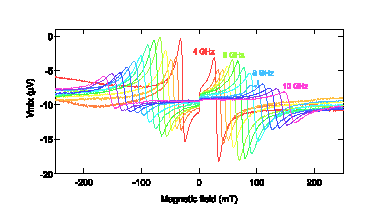
\includegraphics[width=10cm]{images/initial_FMR.eps}
}
\caption{Ni$_{81}$Fe$_{19}$/Pt二層薄膜のST-FMRスペクトル.$4\rm\ GHz$から$10\rm\ GHz$まで$0.5\rm\ GHz$ごとに測定したもの.
}
\label{fig:initial_FMR} 
\end{figure}

この測定したそれぞれのFMRスペクトルをフィッティングすると対称成分$V_{\rm sym}$と反対称成分$V_{\rm asym}$に分離することができる.例えば$7\rm\ GHz$のスペクトルの$V_{\rm sym}$と$V_{\rm asym}$を分離してまとめた結果がFig.\ref{fig:Vseparate}である.\textcolor{blue}{前の章で述べたように}対称成分$V_{\rm sym}$にはdamping-likeトルク,反対称成分$V_{\rm asym}$にはfield-likeトルクの寄与が強く含まれている.この分離をするために強磁性体膜厚依存性が必要である.

Fig.\ref{fig:initial_FMR}の周波数依存性及びフィッティング結果からわかることも多い.

まず共鳴周波数と共鳴磁場の関係からKittelの公式を用いるとNi$_{81}$Fe$_{19}$の飽和磁化が定量できる.その結果がFig.\ref{fig:kittel_initial}である.これらの結果から飽和磁化は$644.29 \pm 0.78\rm\ mT$(正磁場側),$661.56 \pm 1.9\rm\ mT$(負磁場側)と定量できた.



\begin{figure}[htbp]
\centerline{
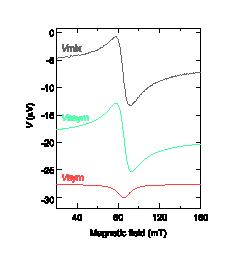
\includegraphics[width=8cm]{images/Vseparate.eps}
}
\caption{Ni$_{81}$Fe$_{19}$/Pt二層薄膜のST-FMRスペクトルに含まれる対称成分$V_{\rm sym}$と反対称成分$V_{\rm asym}$(ただし$7\rm\ GHz$で測定したもの).
}
\label{fig:Vseparate} 
\end{figure}


\begin{figure}[htbp]
\centerline{
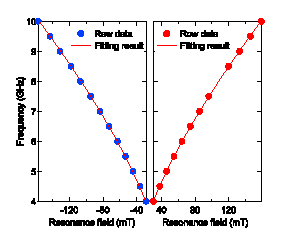
\includegraphics[width=8cm]{images/kittel_initial.eps}
}
\caption{共鳴周波数と共鳴磁場の関係.この関係はKittelの式で表すことができる.青のデータが負磁場,赤のデータが正磁場側の結果である.フィッティング結果はKittelの式の飽和磁化をフィッティングパラメータとしている.
}
\label{fig:kittel_initial} 
\end{figure}

また前に述べたようにスペクトル線幅$W$の周波数依存性から試料のダンピング定数$\alpha$及び不均一線幅が定量できる.スペクトル線幅$W$にはスピン流などのスピン角運動量のダイナミクスによる線幅の変化と強磁性体の不均一性から生じる線幅の変化が含まれる.それらを分離するために周波数依存性を測定した.線幅の周波数依存性の結果はFig.\ref{fig:V-f}に示した.この結果からダンピング及び不均一幅が定量できる.不均一線幅は$0.050\rm\ mT$だった.ここあらこの実験で用いたNi$_{81}$Fe$_{19}$の不均一性は小さいと言える.
\begin{figure}[htbp]
\centerline{
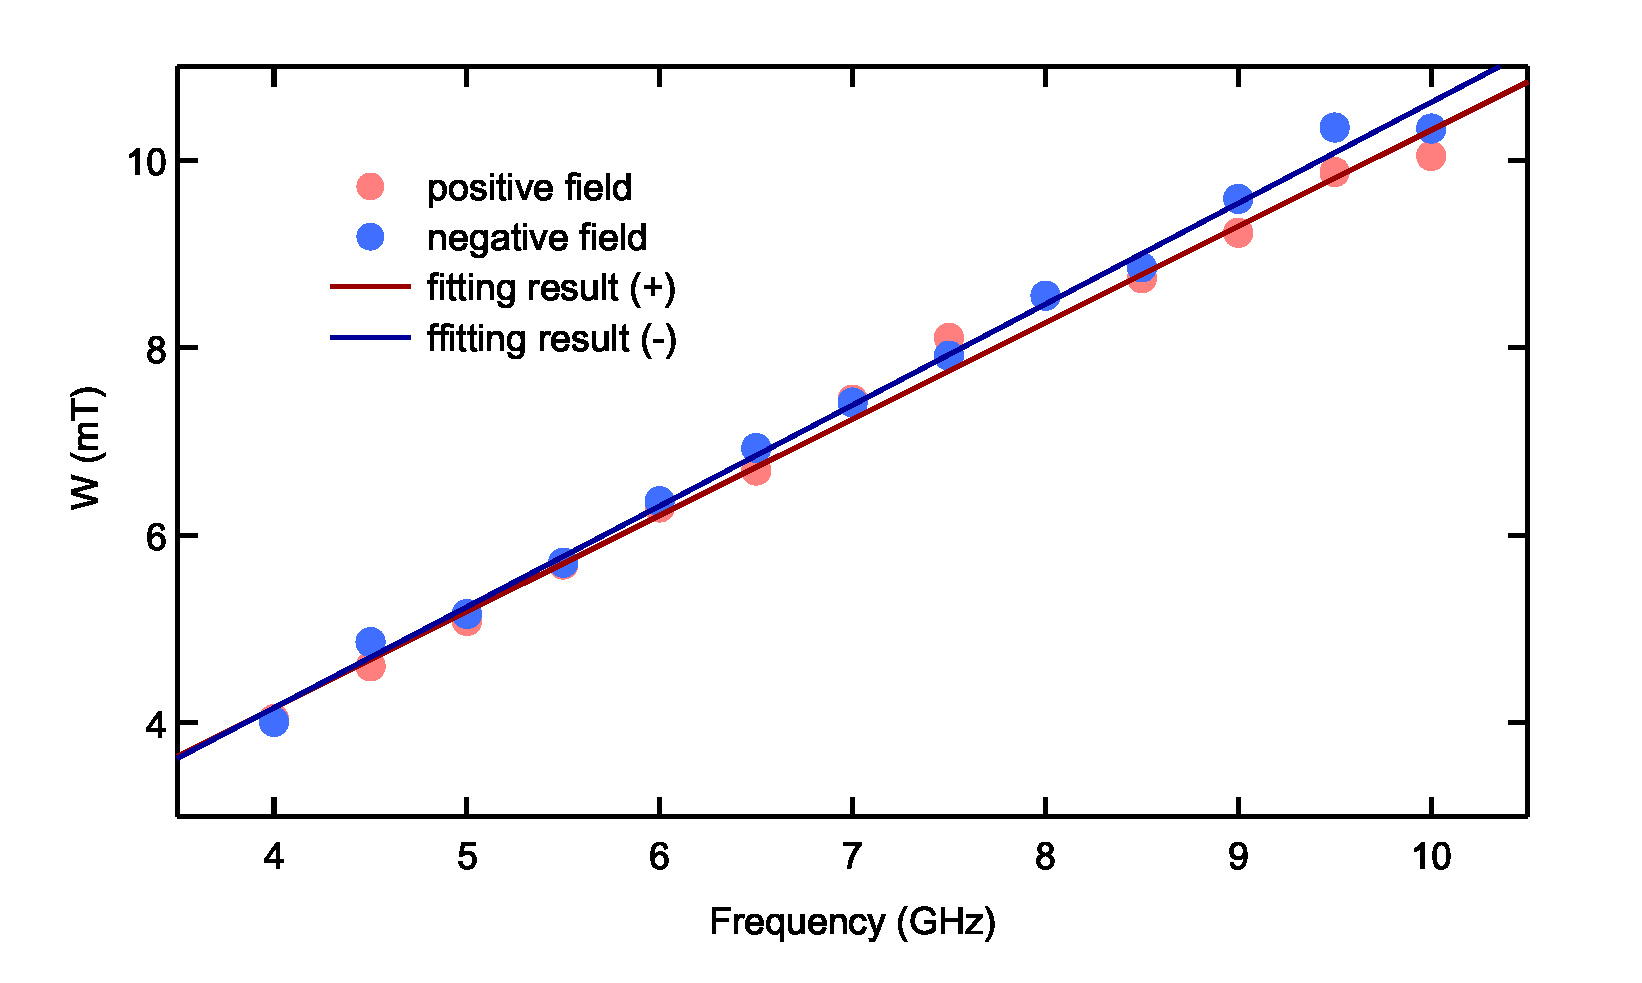
\includegraphics[width=10cm]{images/W-f.eps}
}
\caption{Ni$_{81}$Fe$_{19}$/Pt二層薄膜のスペクトル線幅の周波数依存性.青のデータが負磁場側のスペクトル,赤のデータが正磁場側のスペクトルの結果である.
}
\label{fig:V-f} 
\end{figure}


次にFig.\ref{fig:initial_FMR}の結果から電流-スピン軌道トルク生成効率$\xi_{\rm FMR}$を求めた結果を述べる.スペクトルから$V_{\rm sym}$と$V_{\rm asym}$の比をを求め,Fig.\ref{fig:W-f.eps}から求めた飽和磁化を用いて算出する.まず正磁場及び負磁場のスペクトルから求めた$\xi_{\rm FMR}$はFig.\ref{fig:xi_initial}に示した.ここからPtの$\xi_{\rm FMR}$は0.06程度だと見積れる.この結果は他のグループの報告と一致しており,Ptの$\xi_{\rm FMR}$を再現できていると考えられる.この結果からdamping-likeトルク及びfield-likeトルクの生成効率を見積もるため,Ni$_{81}$Fe$_{19}$の膜厚依存性を測定した.この結果と比較することでイオン液体によるエッチングから求めた結果が妥当なものであるかを検討する.

\begin{figure}[htbp]
\centerline{
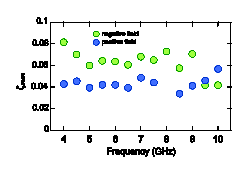
\includegraphics[width=10cm]{images/xi_initial.eps}
}
\caption{Ni$_{81}$Fe$_{19}$/Pt二層薄膜における電流-スピン軌道トルク生成効率$\xi_{\rm FMR}$の周波数依存性.緑の円が負磁場側,青の円が正磁場側のスペクトルから定量した結果.
}
\label{fig:xi_initial} 
\end{figure}




\section{イオン液体によるNi$_{81}$Fe$_{19}$薄膜のエッチング}
\label{sec:PyPt}
この章ではまずイオン液体によってNi$_{81}$Fe$_{19}$をエッチングする方法の模索について述べる.本研究の最初はゲート電圧の印可方向を正方向に設定しエッチングをしていたが,負方向にすることでスムーズなエッチング及びST-FMR測定結果を得られることを発見した.その過程を以下にまとめる.

\subsection{イオン液体による電気化学エッチング -正のゲート電圧-}
本研究は塩貝らが超伝導体をイオン液体の電気化学効果によってエッチングした方法\textcolor{blue}{[]}に着目して始まった.そのためまず塩貝らと同様の方法でイオン液体にゲート電圧を印可した.というのも塩貝らの論文にはFig.\ref{fig:shiogai}のような模式図がありこのゲート電圧の印可方向は一般的なゲート電圧と同方向であるため,本研究でも最初はこのゲート電圧方向を採用した.

\begin{figure}[htbp]
\centerline{
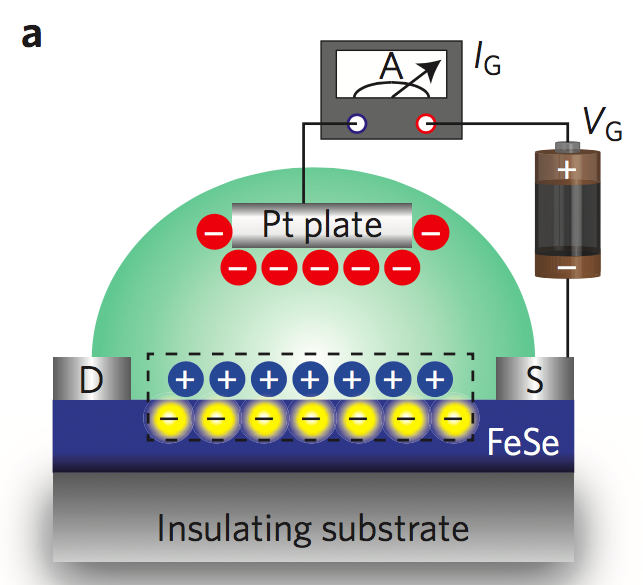
\includegraphics[width=7cm]{images/shiogaireport.png}
}
\caption{塩貝らのイオン液体による超伝導体(FeSe)のエッチング方法の模式図\textcolor{blue}{[]}.エッチングする超伝導体側がゲート電圧の負側になっている.
}
\label{fig:shiogai} 
\end{figure}

本研究ではまずイオン液体によってNi$_{81}$Fe$_{19}$薄膜がエッチングされるのかを確認するために,エッチングのためのゲート電圧を印可しその時の試料の抵抗変化を測定した.このときの測定系はFig.\ref{fig:IL_resi_setup}に示したような回路で表せる.エッチングの可否を点A-B間の抵抗$R_{\rm AB}$の変化によって確認した.ただしこの$R_{\rm AB}$には試料(Ni$_{81}$Fe$_{19}$(8)/Pt(10))の抵抗に加え接触抵抗及び金電極の抵抗が含まれている.

\begin{figure}[htbp]
\centerline{
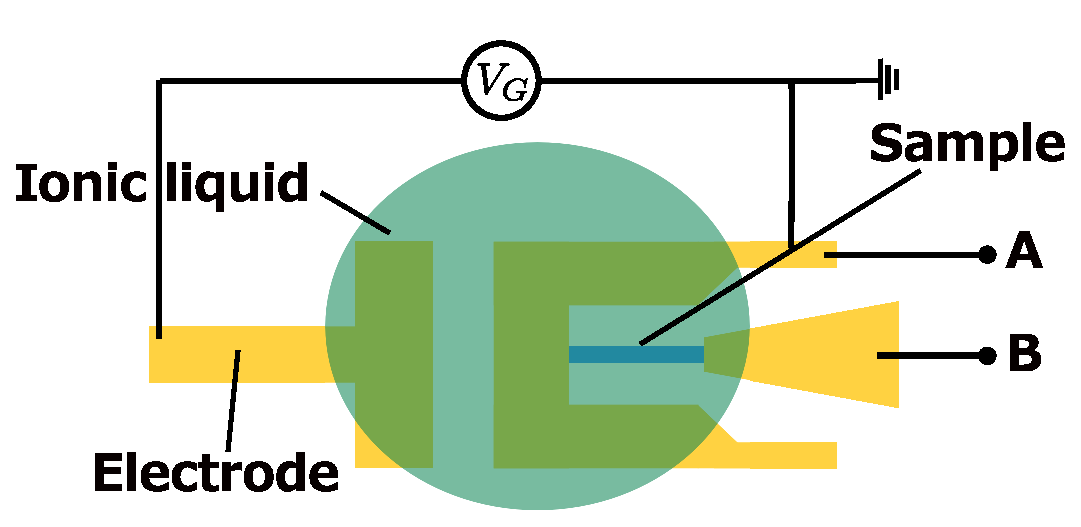
\includegraphics[width=7cm]{images/IL_resi_setup.eps}
}
\caption{ST-FMR測定系での抵抗測定の模式図.点A-B間の抵抗$R_{\rm AB}$を測定しエッチングによるその変化を追跡した.
}
\label{fig:IL_resi_setup} 
\end{figure}



\begin{figure}[htbp]
\centerline{
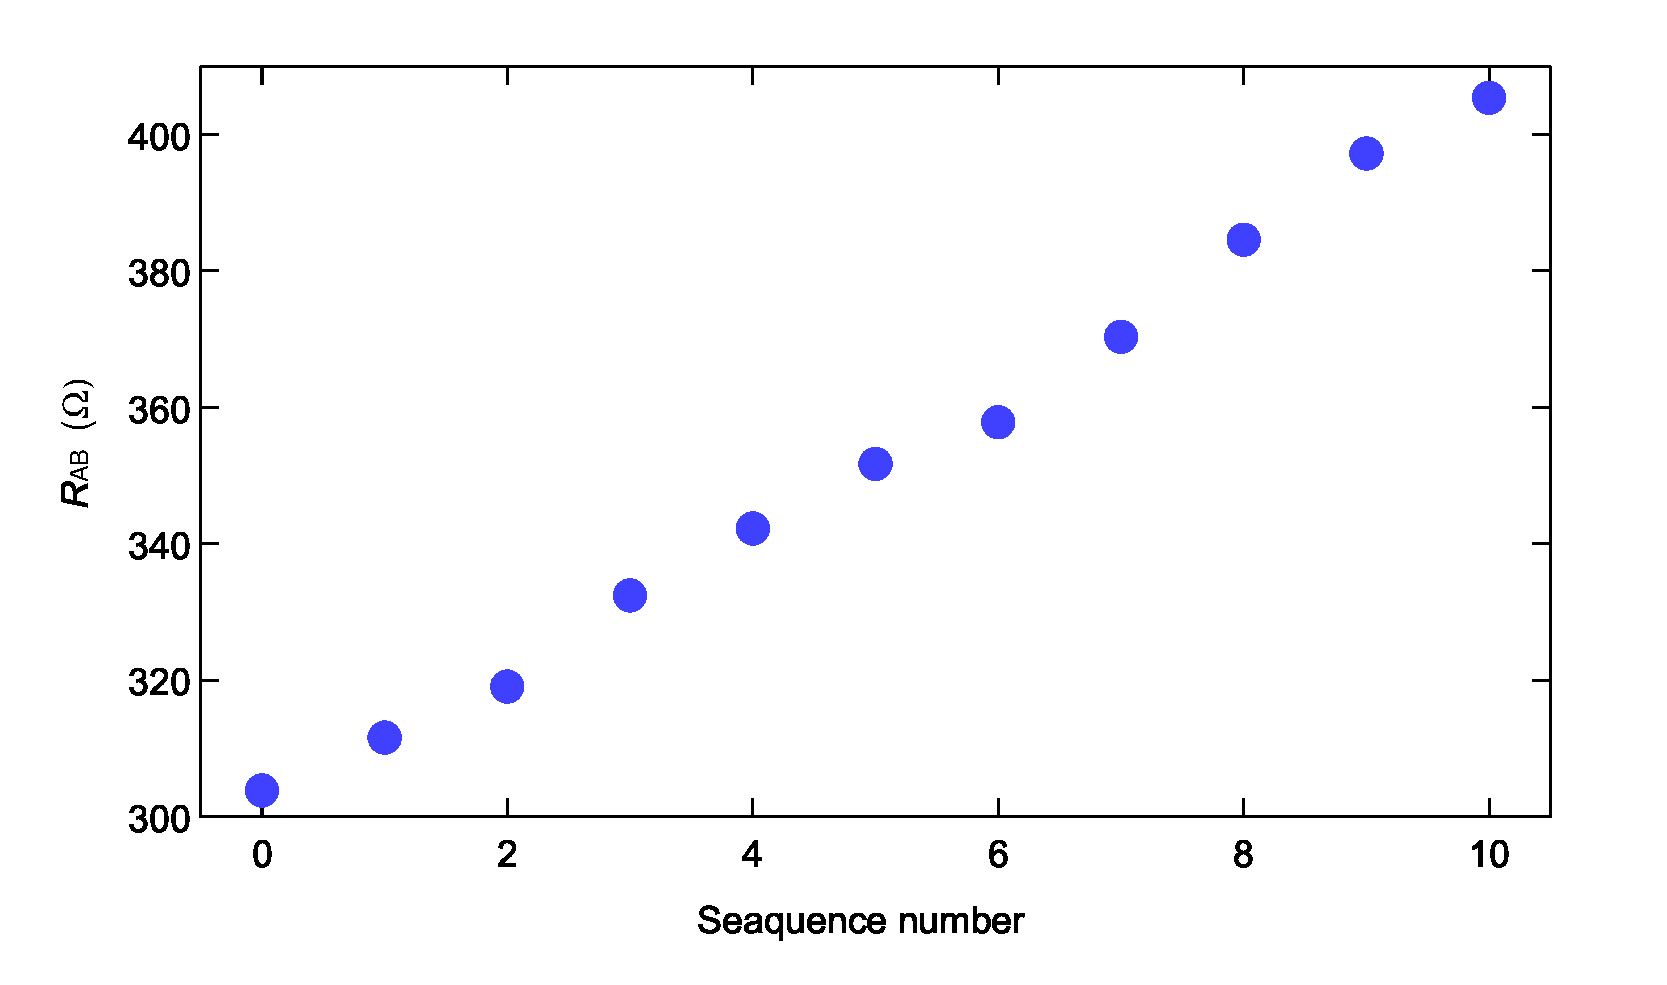
\includegraphics[width=7.5cm]{images/resichange_before.eps}
}
\caption{イオン液体によるエッチングによる$R_{\rm AB}$の変化.イオン液体にゲート電圧5Vを15 sec印可しその後60 sec待機するという操作を一つのシークエンスとしてそれを9回繰り返した結果である.
}
\label{fig:resichange_before} 
\end{figure}

実際にエッチングしながら抵抗測定した結果がFig.\ref{fig:resichange_before}である.x軸のシークエンスというのは,ゲート電圧5 Vを15 sec印可しその後60 sec待機するという流れをエッチングプロセスの一つのシークエンスとしたときの何度エッチングしたかという値である.このときゲート電圧を5 V以下にするとこのような大きな抵抗変化は見られなかった.実際に何時間もの間電圧を印可し続ければエッチングできる可能性もあるが,ある電圧以上でエッチングされる閾値が存在すると推測でき,この結果は他のグループの報告にも一致する.Fig.\ref{fig:resichange_before}を見ると最初の抵抗の値が$303.08\rm \Omega$だったのがエッチングを繰り返すことで$405.5\rm \Omega$と抵抗が増加していることがわかる.ここからイオン液体を用いて実際にNi$_{81}$Fe$_{19}$薄膜の膜厚が減少,つまりエッチングされ得ることが分かった.

そこでこのエッチングを用いてNi$_{81}$Fe$_{19}$/Pt二層薄膜のST-FMR測定を行い,Ni$_{81}$Fe$_{19}$の膜厚依存性を測定した.その結果がFig.\ref{fig:meltingFMR_before}である.

\begin{figure}[htbp]
\centerline{
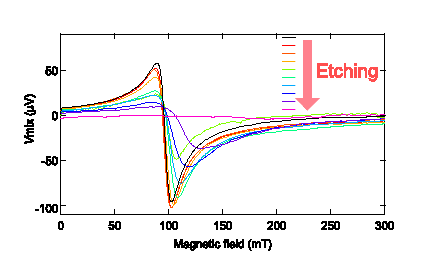
\includegraphics[width=9cm]{images/meltingFMR_before.eps}
}
\caption{イオン液体によるエッチングを利用したFMRの膜厚依存性.黒の線が初期状態を表している.
}
\label{fig:meltingFMR_before} 
\end{figure}

この図を見るとエッチングを進めることによってスペクトルの強度が減少し,さらに線幅及び共鳴磁場が増加していることがわかる.この傾向はNi$_{81}$Fe$_{19}$の膜厚を変えて測定した結果と一致しており,実際にNi$_{81}$Fe$_{19}$がエッチングされていると再確認できる.

そこでFig.\ref{fig:meltingFMR_before}の結果からそれぞれのエッチング後の$\xi_{\rm FMR}$及び$H_{\rm res}$を算出し,それぞれの抵抗から見積もった膜厚に対してプロットした.その結果がFig.\ref{fig:xi_Hreso_d_before}である.

\begin{figure}[htbp]
\centerline{
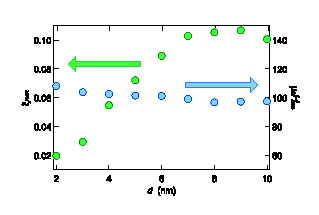
\includegraphics[width=9cm]{images/xi_Hreso_d_before.eps}
}
\caption{エッチングによりNi$_{81}$Fe$_{19}$の膜厚を変化させたときの$\xi_{\rm FMR}$及び$H_{\rm res}$.緑の円が$\xi_{\rm FMR}$を表し,青の円が$H_{\rm res}$を表している.
}
\label{fig:xi_Hreso_d_before} 
\end{figure}


Figure \ref{fig:xi_Hreso_d_before}を見ると$\xi_{\rm FMR}$が膜厚の減少に対して急激に変化している.またそれに対応して共鳴磁場$H_{\rm res}$も変化している.この傾向は他の試料でも再現しており,エッチングによりNi$_{81}$Fe$_{19}$の質が変化してしまっていると考えられる.エッチング前後の試料の光学カメラによる像がFig.\ref{fig:picture_before}である.

\begin{figure}[htbp]
\centerline{
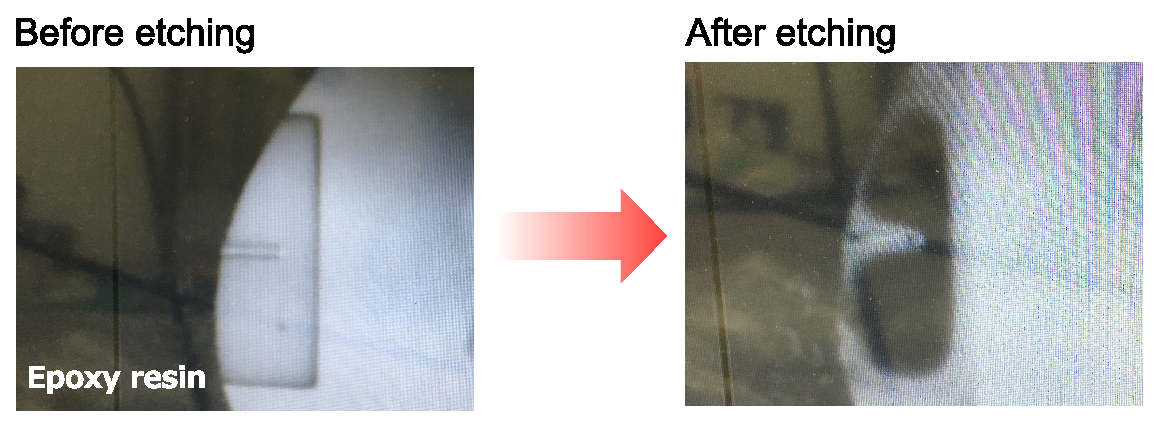
\includegraphics[width=9cm]{images/picture_before.eps}
}
\caption{Ni$_{81}$Fe$_{19}$/Pt二層薄膜のST-FMR試料の光学カメラ像.左の像がエッチング前,右の図がエッチング後の像である.エッチングにより試料から泡のようなものが出ているのがわかる.
}
\label{fig:picture_before}
\end{figure}

この像からわかるようにエッチングによりNi$_{81}$Fe$_{19}$薄膜から泡のようなものが吹き出している.またこの現象は同じゲート電圧を印可していても起きる頻度や量などが異なることから膜が均一に溶けていないことがわかる.

Fig.\ref{fig:xi_Hreso_d_before}の結果から$1/\xi_{\rm FMR}$と$1/d$の関係を計算することはできる.その結果がFig.\ref{fig:xi-1_before}である.

\begin{figure}[htbp]
\centerline{
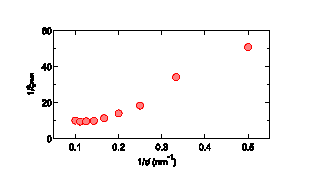
\includegraphics[width=9cm]{images/xi-1_before.eps}
}
\caption{Ni$_{81}$Fe$_{19}$/Pt二層薄膜のST-FMR試料の光学カメラ像.左の像がエッチング前,右の図がエッチング後の像である.エッチングにより試料から泡のようなものが出ているのがわかる.
}
\label{fig:xi-1_before}
\end{figure}

\textcolor{blue}{前章で述べたようにPtの$\xi_{\rm Dl}$及びの$\xi_{\rm FL}$の符号から,$1/\xi_{\rm FMR}$と$1/d$の傾きは負でなければならない.しかしFig.\ref{fig:xi_Hreso_d_before}において$H_{\rm res}$が変化し始めたあたりの膜厚から$1/\xi_{\rm FMR}$の傾きが正に転じている.}つまりこの膜厚付近からNi$_{81}$Fe$_{19}$が違う強磁性体になっている可能性がある.そのためST-FMR測定の設定が異なってしまっていると考えられる.この一つの原因としてあげられるのがNi$_{81}$Fe$_{19}$のNi及びFeの電気陰性度の違いによるエッチング速度の違いである.この差のためにNi$_{81}$Fe$_{19}$薄膜が一様にエッチングされず強磁性体がエッチングによってNi$_{81}$Fe$_{19}$ではないものに変化してしまっている可能性である.この可能性はXPSなどの元素分析で調べて検討しなければならない.\\

ここで再考したのがイオン液体に対するゲート電圧の方向である.通常の電気分解と比較して考える.粗銅の電気精錬を思い出すとFig. \ref{fig:denkibunkai}のように融解させたい物質(ここでは粗銅)を電圧の正側に接続している.

\begin{figure}[htbp]
\centerline{
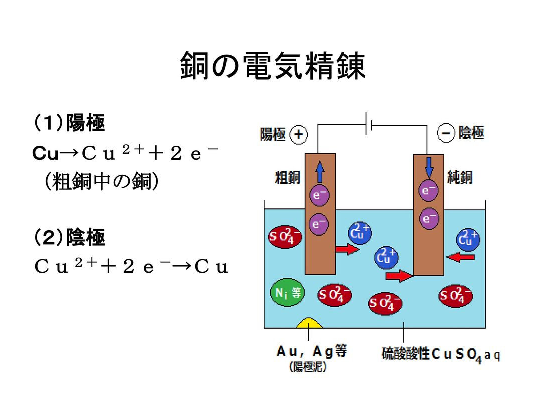
\includegraphics[width=9cm]{images/denkibunkai.eps}
}
\caption{粗銅の電気分解の模式図.溶ける粗銅が電圧の正側に接続している.
}
\label{fig:denkibunkai}
\end{figure}

ここまでの実験設定ではFig.\ref{fig:IL_resi_setup}のように融解させたい(エッチングしたい)試料側が電圧の負側に接続していた.しかしこの条件だと逆に電極側から(e$^{-}$)が引き抜かれ試料側に電子が集まってしまう.この設定でも,上で示したように試料を含んだ電気抵抗$R_{\rm AB}$が増加したことやFMRスペクトルの変化が観測されたことからNi$_{81}$Fe$_{19}$薄膜はエッチングされていたことは明らかである.しかし一方でこの設定では金属が電気化学効果によってイオン化して融解するという現象は起きてない可能性がある.そこで先行研究とはゲート電圧の印可方向が逆になってしまうが,試料側をゲート電圧の正側に接続して上記の実験と同様のエッチングプロセスを行なった.\\

\subsection{イオン液体による電気化学エッチング -負のゲート電圧-}


まずエッチングによりFig.\ref{fig:IL_resi_setup}の抵抗$R_{\rm AB}$がどのように変化するかを観測した.このとき用いた試料はNi$_{81}$Fe$_{19}$(8)/Pt(10)であり,エッチングプロセスはゲート電圧$3\rm\ V$を15 sec,待機時間をが240 secである.それを10シークエンス繰り返した.その結果がFig.\ref{fig:resichange_after}である.

\begin{figure}[htbp]
\centerline{
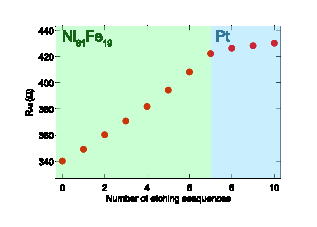
\includegraphics[width=9cm]{images/resichange_after.eps}
}
\caption{イオン液体による電気化学効果を利用したエッチングでの電気抵抗変化.緑の部分がNi$_{81}$Fe$_{19}$が青の部分がPtが溶けている部分だと考えられる.
}
\label{fig:resichange_after}
\end{figure}

Figure.\ref{fig:resichange_after}を見ると緑の領域と青の領域で抵抗変化率が異なっていることがわかる.ここから表面にあるNi$_{81}$Fe$_{19}$が溶け(緑の領域),表面にPtが現れるとPtが溶けることによって(青の領域)抵抗が増加していると推測できる.変化率の違いはNi$_{81}$Fe$_{19}$とPtの電気陰性度の違いを反映しており,Ni$_{81}$Fe$_{19}$よりPtの方が電気陰性度が小さいことと一致している.(\textcolor{blue}{ただしNi$_{81}$Fe$_{19}$の電気陰性度は一般的な合金の電気陰性度の算出の方法を参考にしている[].})

次にこの抵抗と同時に測定したST-FMR測定の結果をFig.\ref{fig:melting_after}に示した.ただしマイクロ波周波数を$7\rm\ GHz$,パワーを$100\rm\ mW$として行なった結果である.

\begin{figure}[htbp]
\centerline{
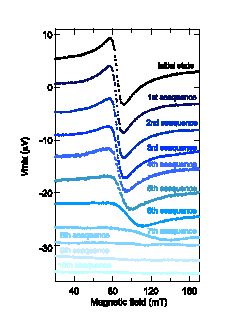
\includegraphics[width=8cm]{images/melting_after.eps}
}
\caption{イオン液体の電気化学効果によってNi$_{81}$Fe$_{19}$/Ptをエッチングした時のFMRスペクトルの変化.一番上のスペクトルが初期状態でそこからエッチングプロセスを繰り返した結果.
}
\label{fig:melting_after}
\end{figure}

このFig.\ref{fig:resichange_after}およびFig.\ref{fig:melting_after}の結果からゲート電圧方向を逆にしてもNi$_{81}$Fe$_{19}$の膜厚を削ることは可能なようである.むしろこのゲート電圧方向の方が均一にNi$_{81}$Fe$_{19}$薄膜がエッチングされているようである.このような推測は以下のような議論から考えられる.Figure.\ref{fig:melting_after}とFig.\ref{fig:meltingFMR_before}を比較すると共鳴磁場の変化が異なっている.前者はかなりエッチングが進行した後に共鳴磁場が変化しているのに対し,後者はエッチング初期から共鳴磁場のシフトが見られる.Ni$_{81}$Fe$_{19}$の膜厚を薄くすると飽和磁化が減少することは知られており[\textcolor{blue}{引用したほうがいい}],Fig.\ref{fig:melting_after}の共鳴磁場の変化はこの強磁性体も膜厚が極めて薄くなった影響を反映していると考えられる.対してFig.\ref{fig:meltingFMR_before}の結果はエッチングを始めた直後から共鳴磁場が変化しており,エッチングによるNi$_{81}$Fe$_{19}$の変化による共鳴磁場の変化も含まれると思われる.ここからゲート電圧の方向を負にした設定の方が強磁性薄膜が均一に溶けていると考えられる.

共鳴磁場の変化をFig.\ref{fig:resichange_after}の解析可能なスペクトルから算出するとFig.\ref{fig:Hreschange_after}の緑の円のようになる.またFMRスペクトルの周波数依存性から初期状態の飽和磁化$\mu_{0}M_{\rm s} = 664.29\rm\ mT$を出し,この初期状態の飽和磁化の値と共鳴磁場からKittelの式を用いてそれぞれの共鳴磁場に対応する飽和磁化を求めた値が\ref{fig:Hreschange_after}の青の円である.

\begin{figure}[htbp]
\centerline{
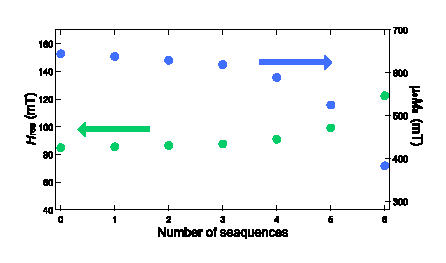
\includegraphics[width=10cm]{images/Hreschange_after.eps}
}
\caption{イオン液体の電気化学効果によってNi$_{81}$Fe$_{19}$/Ptをエッチングしたときの共鳴磁場及び飽和磁化の変化.
}
\label{fig:Hreschange_after}
\end{figure}

エッチングプロセスを7回以上繰り返すとFig.\ref{fig:resichange_after}の青の領域に入り,Fig.\ref{fig:melting_after}でもわかるようにFMRのスペクトルが観測できなくなる.上でも述べたように共鳴磁場がシークエンスの後半で大きく変化している.これはNi$_{81}$Fe$_{19}$の膜厚が薄くなることに連れて飽和磁化が小さくなることを示している.



ここでエッチングしたときの膜厚を求めたい.そのためにエッチング前と後のAFMを用いた試料の膜厚測定を行なった.その結果がFig.\ref{fig:AFMpicture}である.この測定から分かったバーの厚さは表\ref{table:AFM}のようになった.

\begin{figure}[htbp]
\centerline{
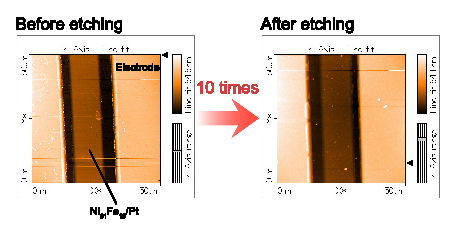
\includegraphics[width=11cm]{images/AFMpicture.eps}
}
\caption{エッチングプロセス前後のNi$_{81}$Fe$_{19}$/Pt薄膜試料のAFM像.像の中心にあるバー状のものが試料,それの周りにある部分が電極である.
}
\label{fig:AFMpicture}
\end{figure}


\begin{table}[hbtp]
  \caption{Ni$_{81}$Fe$_{19}$/Pt薄膜のエッチング前後の膜厚.Ptはほとんどエッチングされていないとすると}
  \label{table:AFM}
  \centering
  \begin{tabular}{lcr}
    \hline
           &   Before etching   & After etching  \\
    \hline \hline
    Ni$_{81}$Fe$_{19}$/Pt  & $17.03\rm\ nm$  & $9.63\rm\ nm$ \\
    \hline
  \end{tabular}
\end{table}

一方Fig.\ref{fig:resichange_after}からエッチングによる抵抗$R_{\rm AB}$の変化はわかる.この$R_{\rm AB}$には試料の抵抗だけでなく接触抵抗及び金電極の抵抗も含んでいる.Ni$_{81}$Fe$_{19}$/Pt二層薄膜の抵抗がそれぞれの層の抵抗$R_{\rm Ni$_{81}$Fe$_{19}$}$及び$R_{\rm Pt}$の並列回路で再現できると仮定し,試料以外の抵抗(接触抵抗及び金電極の抵抗など)を$R_{\rm ex}$とすると$R_{\rm AB}$は

\begin{eqnarray}
R_{\rm AB} = \frac{R_{\rm Ni_{81}Fe_{19}}R_{\rm Pt}}{R_{\rm Ni_{81}Fe_{19}}+R_{\rm Pt}} + R_{\rm ex}
\label{eq:RAB}
\end{eqnarray}
となる.この式\ref{eq:RAB}の関係に Ni$_{81}$Fe$_{19}$の厚さ$d$を含めて$d$を$R_{\rm AB}$で表したい.そのために個別で調べた表\ref{table:resi}の物性値を用いて$R_{\rm AB}$を$d$と$R_{\rm AB}$の関数とした式が式\ref{eq:RAB2}である.

\begin{table}[hbtp]
  \caption{Ni$_{81}$Fe$_{19}$およびPtの物性値.}
  \label{table:resi}
  \centering
  \begin{tabular}{ccc}%lが左cが中央rが右揃えって意味
    \hline
           &   Ni$_{81}$Fe$_{19}$   & Pt  \\
    \hline \hline
   electrical resistivity  & $1.057\times10^{-6}\rm\ \Omega\cdot m$  & $3.00\times10^{-7}\rm\ \Omega\cdot m$\\
   thickness  &  $d\rm\ nm$  &  $10\rm\ nm$\\
   length  &  $130\rm\ \mu m$  &  $130\rm\ \mu m$\\
   width  &  $10\rm\ \mu m$   &  $10\rm\ \mu m$\\
    \hline
  \end{tabular}
\end{table}


\begin{eqnarray}
R_{\rm AB} = \frac{1}{\frac{1}{390}+7.277\times10^{4}d} + R_{\rm ex}
\label{eq:RAB2}
\end{eqnarray}

まず測定結果から$R_{\rm AB}$の値を求めて式\ref{eq:RAB2}から取り除きたい.そうすれば$d$が$R_{\rm AB}$だけの関数になり,Fig.\ref{fig:resichange_after}の結果からそれぞれのNi$_{81}$Fe$_{19}$の膜厚が見積れる.
Figure.\ref{fig:resichange_after}の緑と青の領域の境界でNi$_{81}$Fe$_{19}$の膜厚が$0\rm\ nm$になったと仮定すると,この境界における抵抗$R_{\rm AB}(d=0\rm\ nm)$はPtと$R_{\rm ex}$だけで表せる.表\ref{table:resi}の物性値を用いたPt単層の抵抗は$390\rm \Omega$になるはずだが,$R_{\rm AB}(d=0\rm\ nm) = 422.09\rm\ \Omega$である.この差$422.09-390 = 32.09\rm\ \Omega$が$R_{\rm ex}$と考えられる.この$R_{\rm ex}$はエッチングによって変化しないと考えられるので,$R_{\rm ex}$をFig.\ref{fig:resichange_after}の全体の測定結果から引く.その結果がFig.\ref{fig:RAB-Rex}である.


\begin{figure}[htbp]
\centerline{
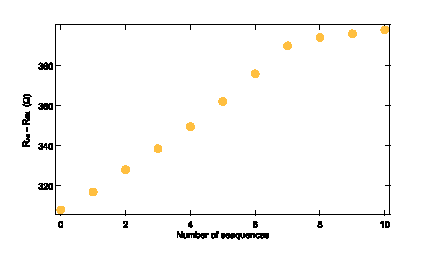
\includegraphics[width=9cm]{images/RAB-Rex.eps}
}
\caption{$R_{\rm AB}-R_{\rm ex}$のエッチングによる変化.
}
\label{fig:RAB-Rex}
\end{figure}

式\ref{eq:RAB2}を変形すると式\ref{eq:d}となる.

\begin{eqnarray}
d = \frac{1}{7.277\times10^{4}}\left(\frac{1}{R_{\rm AB} - R_{\rm ex}}-\frac{1}{390}\right)
\label{eq:d}
\end{eqnarray}
この計算をFig.\ref{fig:RAB-Rex}に適応し$d$を求めたのがFig.\ref{fig:d_after}である.

\begin{figure}[htbp]
\centerline{
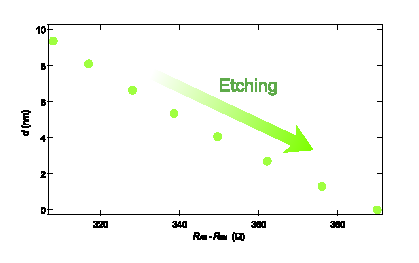
\includegraphics[width=9cm]{images/d_after.eps}
}
\caption{$R_{\rm AB}-R_{\rm ex}$から計算した$d$.シークエンス7以降はNi$_{81}$Fe$_{19}$が溶けた後なので示していない.
}
\label{fig:d_after}
\end{figure}

こうして見積もった膜厚$d$と$\xi_{FMR}$の関係をプロットしたものがFig.\ref{fig:xi-1_after}である.この傾き及び切片から$\xi_{\rm DL}$及び$\xi_{\rm FL}$が算出できる.

\begin{figure}[htbp]
\centerline{
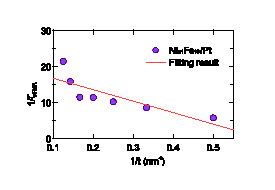
\includegraphics[width=10cm]{images/xi-1_after.eps}
}
\caption{イオン液体の電気化学効果を用いて求めた$\xi_{\rm FMR}^{-1}$と$t^{-1}$の関係.
}
\label{fig:xi-1_after}
\end{figure}

Figure.\ref{fig:xi-1_after}から見積もった$\xi_{\rm DL}$及び$\xi_{\rm FL}$を表\ref{table:xi}に示した.比較対象として本研究室で異なるNi$_{81}$Fe$_{19}$の膜厚を持った試料を作成し定量した値と他のグループが定量した値を記載した.


\begin{table}[hbtp]
  \caption{Ni$_{81}$Fe$_{19}$/Ptの$\xi_{\rm DL}$及び$\xi_{\rm FL}$.}
  \label{table:xi}
  \centering
  \begin{tabular}{ccc}%lが左cが中央rが右揃えって意味
    \hline
           &   $\xi_{\rm DL}$   & $\xi_{\rm FL}$  \\
    \hline \hline
   Etched with IL  & $0.0347 $  & $-0.322$\\
   Prepared each samples  &    &  \\
   \textcolor{blue}{Reference[]}  & $0.100\pm 0.005$  & $-0.004\pm 0.003$\\
    \hline
  \end{tabular}
\end{table}


表\ref{table:xi}でわかるように$\xi_{\rm DL}$及び$\xi_{\rm FL}$は膜厚を変えた試料を複数用意して定量した値と本研究の結果とでそれぞれ誤差がある.$\xi_{\rm DL}$はFig.\ref{fig:xi-1_after}における切片の逆数と同値である.エッチング初期におけるフィッティング誤差が大きく影響を及ぼしていると考えられる.また膜厚を算出する際に抵抗率が一定であるという過程を用いている.\textcolor{blue}{しかし実際は膜厚が薄くなるにつれて薄膜の表面散乱の影響が大きくなり低効率の増加が見られる[].}その効果を無視している影響も考えられる.



\section{まとめ}
本研究で得られた主要な結果は以下の2点である。
\begin{enumerate}
 \item Ni$_{81}$Fe$_{19}$/Pt二層薄膜におけるST-FMR測定の強磁性体膜厚依存性を測定した.
 \item イオン液体の電気化学効果を用いたエッチング方法を確立し,単一の試料を用意するだけでST-FMR測定の強磁性体膜厚依存性を測定可能にした.
\end{enumerate}
